\epi{Go 有指针,但是没有指针运算。你不能用指针变量遍历字符串的各个字节。
}{\textit{Go For C++
Programmers}\\{\textsc{GO AUTHORS}}}
\noindent{}
Go 有指针。然而却没有指针运算,因此它们更象是引用而不是你所知道的来自于 C 的指针。
指针非常有用。
在 Go 中调用函数的时候,得记得变量是\emph{值传递}的。
因此,为了修改一个传递\emph{入}函数的值的效率和可能性,有了指针。

跟 C 中一样,用类型前的 '\key{*}' 定义一个指针:
\lstinline{var p *int}。现在 \var{p} 是一个指向整数值的指针。
所有新定义的变量都被赋值为其类型的零值,而指针也一样。
一个新定义的或者没有任何指向的指针,有值 \first{nil}{nil}。
在其他语言中,这经常被叫做空(NULL)指针,在 Go 中就是 \var{nil}。
让指针指向某些内容,可以使用\first{取址操作符}{operator!address-of}
(\func{\&}),像第 5 行那样:
\begin{lstlisting}[caption=Use of a pointer,label=src:pointers]
var p *int
fmt.Printf("%v", p) |\coderemark{打印 \var{nil}}|

var i int	    |\coderemark{定义一个整形变量 \var{i}}|
p = &i		    |\coderemark{使得 \var{p} 指向 \var{i}}|

fmt.Printf("%v", p) |\coderemark{打印出来的内容类似 \var{0x7ff96b81c000a}}|
\end{lstlisting}

更简单来说:\var{*X} 是指向 \type{X} 的指针;\var{[3]X} 是有三个 \type{X} 的数组。
因此类型更加容易从类型变化的名称上来理解:
\type{[]} 定义了 slice;
'\key{*}'
定义了指针;
\type{[size]} 定义了数组。因此 \type{[]*[3]*X} 是一个 slice,
元素是指向有三个元素的数组的指针,数组元素是指向 \type{X} 的指针。
(参阅 \ref{fig:pointers})。
\begin{figure}[h]
\caption[Pointers and types]{指针和类型,值 \var{v} 全部为 \type{X} 类型}
\label{fig:pointers}
\begin{center}
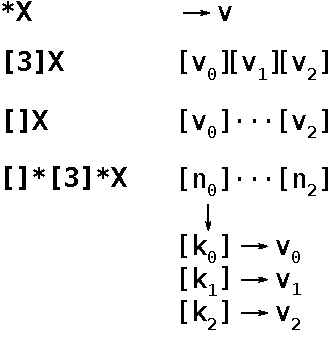
\includegraphics[scale=0.65]{fig/pointers.pdf}
\end{center}
\end{figure}

从指针获取值是通过在指针变量前置'\type{*}'实现的:
\begin{lstlisting}[caption=获取指针指向的值,label=src:deref]
p = &i			|\coderemark{获取 \var{i} 的地址}|
*p = 8			|\coderemark{修改 \var{i} 的值}|
fmt.Printf("%v\n", *p)  |\coderemark{打印 8}|
fmt.Printf("%v\n", i)	|\coderemark{同上}|
\end{lstlisting}

前面已经说了,没有指针运算,所以如果这样写:
\lstinline{*p++},它表示 \lstinline{(*p)++}:首先获取指针指向的值,然后对这个值加一。
\index{operator!increment}


\section{内存分配}
Go 有垃圾收集,意味着无须担心内存分配和回收。当然,自从 1980 以来几乎所有语言都有这个,
但是在类 C 语言中看到垃圾收集感觉还是很好。

Go 有两个内存分配原语,\key{new} 和 \key{make}。它们应用于不同的类型,做不同的工作,
可能有些迷惑人,但是规则很简单。
下面的章节展示了在 Go 中如何处理内存分配,并且希望能够让
\first{\key{new}}{built-in!new} 和 \first{\key{make}}{built-in!make} 之间的区别更加清晰。

\subsection{用 new 分配内存}
\label{sec:allocation with new}
内建函数 \key{new} 本质上说跟其他语言中的同名函数功能一样:
\func{new(T)} 分配了零值填充的 \type{T} 类型的内存空间,并且返回其地址,
一个 \type{*T} 类型的值。用 Go 的术语说,它返回了一个指针,指向新分配的类型 \type{T}
的零值。有一点非常重要:
\begin{lbar}
\key{new} 返回\emph{指针}。
\end{lbar}

这意味着使用者可以用 \key{new} 创建一个数据结构的实例并且可以直接工作。
如 \func{bytes.Buffer} 的文档所述“Buffer 的零值是一个准备好了的空缓冲。”
类似的,\func{sync.Mutex} 也没有明确的构造函数或 Init 方法。取而代之,
\func{sync.Mutex} 的零值被定义为非锁定的互斥量。

零值是非常有用的。例如这样的类型定义,\pageref{sec:defining your own}
页的 "\titleref{sec:defining your own}" 内容。
\begin{lstlisting}
type SyncedBuffer struct {
    lock    sync.Mutex
    buffer  bytes.Buffer
}
\end{lstlisting}
\type{SyncedBuffer} 的值在分配内存或定义之后立刻就可以使用。在这个片段中,
\var{p} 和 \var{v} 都可以在没有任何更进一步处理的情况下工作。
\begin{lstlisting}
p := new(SyncedBuffer)  |\coderemark{Type *SyncedBuffer}|
var v SyncedBuffer      |\coderemark{Type  SyncedBuffer}|
\end{lstlisting}

\subsection{用 make 分配内存}
\label{sec:allocation with make}
回到内存分配。内建函数 \func{make(T, args)} 与 \func{new(T)} 有着不同的功能。
它只能创建 slice,map 和 channel,并且返回一个有初始值(非零)的 \type{T} 类型,
而不是 \type{*T}。本质来讲,
导致这三个类型有所不同的原因是指向数据结构的引用在使用前必须被初始化。
例如,一个 slice,是一个包含指向数据(内部 array)的指针,长度和容量的三项描述符;
在这些项目被初始化之前,slice 为 \type{nil}。对于 slice,map 和 channel,
\key{make} 初始化了内部的数据结构,填充适当的值。

\begin{lbar}
\key{make} 返回初始化后的(非零)\emph{值}。
\end{lbar}

例如,
\lstinline{make([]int, 10, 100)}
分配了 100 个整数的数组,然后用长度 10 和容量 100 创建了 slice 
结构指向数组的前 10 个元素。
区别是,\lstinline{new([]int)} 返回指向新分配的内存的指针,
而零值填充的 slice 结构是指向 \type{nil} 的 slice 值。

这个例子展示了 \key{new} 和 \key{make} 的不同。
\begin{lstlisting}
var p *[]int = new([]int)       // 分配 slice 结构内存;*p == nil
				// 已经可用
var v  []int = make([]int, 100) // v 指向一个新分配的有 100 个整数的数组。

// 不必要的复杂例子:
var p *[]int = new([]int)
*p = make([]int, 100, 100)

// 更常见:
v := make([]int, 100)
\end{lstlisting}
务必记得 \key{make} 仅适用于 map,slice 和 channel,并且返回的不是指针。
应当用 \key{new} 获得特定的指针。

\subsection{Constructors and composite literals}
Sometimes the zero value isn't good enough and an initializing
constructor is necessary, as in this example taken from the package
\package{os}.
\begin{lstlisting}
func NewFile(fd int, name string) *File {
    if fd < 0 {
        return nil
    }
    f := new(File)
    f.fd = fd
    f.name = name
    f.dirinfo = nil
    f.nepipe = 0
    return f
}
\end{lstlisting}
There's a lot of boiler plate in there. We can simplify it using a
composite literal, which is an expression that creates a new instance
each time it is evaluated.

\begin{lstlisting}
func NewFile(fd int, name string) *File {
    if fd < 0 {
        return nil
    }
    f := File{fd, name, nil, 0}	|\coderemark{Create a new \type{File}}|
    return &f			|\coderemark{Return the address of \var{f}}|
}
\end{lstlisting}
It is OK to return the address of a local variable;
the storage associated with the variable survives after the function
returns.

In fact, taking the address of a composite literal allocates a
fresh instance each time it is evaluated, so we can combine these last
two lines.\footnote{Taking the address of a composite literal tells the 
compiler to allocate it on the heap, not the stack.}
\begin{lstlisting}
return &File{fd, name, nil, 0}
\end{lstlisting}
The fields of a composite literal are laid out in order and must all be
present. However, by labeling the elements explicitly as field:value
pairs, the initializers can appear in any order, with the missing ones
left as their respective zero values. Thus we could say

\begin{lstlisting}
return &File{fd: fd, name: name}
\end{lstlisting}
As a limiting case, if a composite literal contains no fields at all, it
creates a zero value for the type. The expressions
\lstinline{new(File)} and 
\lstinline|&File{}| are equivalent.

Composite literals can also be created for arrays, slices, and maps,
with the field labels being indices or map keys as appropriate. In these
examples, the initializations work regardless of the values of
\var{Enone},
\var{Eio}, and \var{Einval}, as long as they are distinct.
\begin{lstlisting}
ar := [...]string   {Enone: "no error", Eio: "Eio", Einval: "invalid argument"}
sl := []string      {Enone: "no error", Eio: "Eio", Einval: "invalid argument"}
ma := map[int]string{Enone: "no error", Eio: "Eio", Einval: "invalid argument"}
\end{lstlisting}

\section{Defining your own types}
\label{sec:defining your own}
Of course Go allows you to define new types, it does this 
with the \first{\key{type}}{keyword!type} keyword: 
\begin{lstlisting}
type foo int
\end{lstlisting}
Creates
a new type \lstinline{foo} which acts like an \lstinline{int}.
Creating more sophisticated types is done with the
\first{\key{struct}}{keyword!struct}
keyword.
An example would be when we want record somebody's name (\type{string})
and age (\type{int}) in a single structure and make it a new type:
\lstinputlisting[label=src:struct,caption=Structures]{src/struct.go}
Apropos, the output of \lstinline{fmt.Printf("%v\n", a)} is 
\begin{display}
&\{Pete 42\}
\end{display}
That is nice!
Go knows how to print your structure. If you
only want to print one, or a few, fields of the structure you'll
need to use \verb|.<field name>|. For example to only print the name:
\begin{lstlisting}
fmt.Printf("%s", a.name) |\coderemark{\%s formats a string}|
\end{lstlisting}

\subsection{More on structure fields}
Each item in a structure is called a field. 
A struct with no fields:
\begin{lstlisting}
struct {}
\end{lstlisting}
One with five fields:
\begin{lstlisting}
struct {
        x, y int
        _ float64  |\coderemark{padding}|
        A *[]int
        F func()
}
\end{lstlisting}
If you omit the name for a field, you create an anonymous field, for
instance:
\begin{lstlisting}
struct {
        T1        // field name is T1
        *T2       // field name is T2
        P.T3      // field name is T3
        x, y int  // field names are x and y
}
\end{lstlisting}
Note the field names that start with a capital letter are exported, i.e. can be
set or read from other packages. Field names that start with a lowercase are private
to the current package. The same goes for functions defined in packages, see chapter
\ref{chap:packages}.

\subsection{Methods}
\label{sec:methods}
If you create functions that works on your newly defined type, you can
take two routes:
\begin{enumerate}
\item Create a function that takes the type as an argument.
\begin{lstlisting}
func doSomething(in1 *NameAge, in2 int) { /* ... */ }
\end{lstlisting}
This is (you might have guessed) a \first{\emph{function call}}{function!call}.
\item Create a function that works on the type (see \emph{receiver} in
listing \ref{src:function definition}):
\begin{lstlisting}
func (in1 *NameAge) doSomething(in2 int) { /* ... */ }
\end{lstlisting}
This is a \first{\emph{method call}}{method call}, which can be
used as: 
\begin{lstlisting}
var n *NameAge
n.doSomething(2)
\end{lstlisting}
\end{enumerate}
But keep the following in mind, this is quoted from \cite{go_spec}:
\begin{quote}
If \type{x} is
addressable and \lstinline{&x}'s method set contains \func{m}, 
\lstinline{x.m()} is shorthand for \lstinline{(&x).m()}.
\end{quote}
In the above case this means that the following is \emph{not} an 
error:
\begin{lstlisting}
var n NameAge	    |\coderemark{Not a pointer}|
n.doSomething(2)    
\end{lstlisting}
Here Go will search the method list for \var{n} of type \type{NameAge},
come up empty and will then \emph{also} search the method list for
the type \type{*NameAge} and will translate this call to
\lstinline{(&n).doSomething(2)}.

\section{Conversions}
\label{sec:conversions}
Sometimes you want to convert a type to another type. 
This is possible in Go, but
there are some rules. For starters, converting from one value to another
is done by functions and not all conversions are allowed.

\begin{table}[H]
\begin{center}
\caption[Valid conversions]{Valid conversions, 
\lstinline{float64} works the same as \lstinline{float32}}
\label{tab:convesion}
\begin{tabular}{llllllll}
    \textbf{From}	 &  \verb|xb []byte|& \verb|xi []int| & \verb|xr []rune| & \verb|s string|     & \verb|f float32|	&  \verb|i int|	\\ \cmidrule(r){1-7}
      \textbf{To}	 &		    &                 &   &			   &			& \\ \cmidrule(r){1-1}
  \verb|[]byte|    & $\texttimes$	    &                 &   & \verb|[]byte(s)|	   &			& \\
  \verb|[]int|     &		    & $\texttimes$            &   & \verb|[]int(s)|	   &			& \\
  \verb|[]rune|    &                &                         & $\texttimes$  &  \verb|[]rune(s)| &                    & \\
  \verb|string|    &\verb|string(xb)| &\verb|string(xi)|      &  \verb|string(xr)| &	$\texttimes$	   &			& \\
 \verb|float32|	 &		    &                         &   &			   & $\texttimes$	& \verb|float32(i)|\\
     \verb|int|	 &		    &                         &   &			   & \verb|int(f)|	& $\texttimes$ \\
%%\bottomrule
\end{tabular}

\end{center}
\end{table}

\begin{itemize}
\item{
From a \lstinline{string} to a slice of bytes or ints.
\begin{lstlisting}
mystring := "hello this is string"
\end{lstlisting}

\begin{lstlisting}
byteslice := []byte(mystring)
\end{lstlisting}
Converts to a \type{byte} slice, each \type{byte} contains the integer value
of the corresponding byte in the string. Note that as strings in Go
are encoded in UTF-8 some characters in the string may end up in 1, 2, 3
or 4 bytes.
\begin{lstlisting}
intslice  := []int(mystring)
\end{lstlisting}
Converts to an \type{int} slice, each \type{int} contains a Unicode code
point. Every character from the string is corresponds to one integer.
}
\item{
From a slice of bytes or ints to a \lstinline{string}.
\begin{lstlisting}
b := []byte{'h','e','l','l','o'} |\coderemark{Composite literal}|
s := string(b)
i := []int{257,1024,65} 
r := string(i)
\end{lstlisting}
}
\end{itemize}
For numeric values the following conversion are defined:
\begin{itemize}
\item{Convert to a integer with a specific (bit) length: 
\lstinline{uint8(int)};}
\item{From floating point to an integer value: 
\lstinline{int(float32)}. This discards the fraction part
from the floating point value;}
\item{The other way around: \lstinline{float32(int)};}
\end{itemize}

\subsection{User defined types and conversions}
How can you convert between the types you have defined
yourself?
We create two types here \type{Foo} and \type{Bar}, where
\lstinline{Bar} is an alias for \type{Foo}:
\begin{lstlisting}
type foo struct { int }  |\coderemark{anonymous struct field}|
type bar foo             |\coderemark{bar is an alias for foo}|
\end{lstlisting}

Then we:
\begin{lstlisting}
var b bar = bar{1} |\coderemark{Declare \var{b} to be a \type{bar}}|
var f foo = b	   |\coderemark{Assign \var{b} to \var{f}}|
\end{lstlisting}
Which fails on the last line with:

\noindent\error{cannot use b (type bar) as type foo in assignment}

\noindent{}This can be fixed with a conversion:
\begin{lstlisting}
var f foo = foo(b)
\end{lstlisting}
Note the converting structures that are not identical in their fields
is more difficult. Also note that converting \lstinline{b} to a plain
\type{int} also fails; an integer is not the same as a structure containing
an integer.

\section{Exercises}
\begin{Exercise}[title={使用 interface 的 map 函数},difficulty=6]
\label{ex:map function interfaces}
\Question
使用练习 Q\ref{ex:map function} 的答案,利用 interface 使其更加通用。
\end{Exercise}

\begin{Answer}
\Question
\lstinputlisting[label=src:map,caption=Go 中更加通用的 map 函数]{ex-beyond/src/map.go}
\end{Answer}




\begin{Exercise}[title={指针},difficulty=6]
\label{ex:pointers}

\Question
假设定义了下面的结构:
\begin{lstlisting}
type Person struct {
    name string
    age	 int
}
\end{lstlisting}

下面两行之间的区别是什么?
\begin{lstlisting}
var p1 Person
p2 := new(Person)
\end{lstlisting}

\Question
下面两个内存分配的区别是什么?
\begin{lstlisting}[numbers=none]
func Set(t *T) {
    x = t
}
\end{lstlisting}
和
\begin{lstlisting}[numbers=none]
func Set(t T) {
    x= &t
}
\end{lstlisting}
\end{Exercise}

\begin{Answer}
\Question
第一行:\lstinline{var p1 Person} 分配了
\texttt{Person}-\emph{值} 给 \var{p1}。\var{p1} 的类型是
\type{Person}。

第二行:\lstinline{p2 := new(Person)} 分配了内存并且将\emph{指针}赋值给
\var{p2}。\var{p2} 的类型是 \type{*Person}。

\Question
在第二个函数中,\var{x} 指向一个新的(堆上分配的)变量
\var{t},其包含了实际参数值的副本。

在第一个函数中,\var{x} 指向了 \var{t} 指向的内容,
也就是实际上的参数指向的内容。

因此在第二个函数,我们有了``额外''的变量存储了相关值的副本。
\end{Answer}


\begin{Exercise}[title={Linked List},difficulty=1]
\label{ex:linkedlist}
\Question
\label{ex:linkedlist q1}
Make use of the package \package{container/list} to create
a (double) linked list. Push the values 1, 2 and 4 to the list and then
print it.

\Question
Create your own linked list implementation. And perform the same actions
as in question \ref{ex:linkedlist q1}
\end{Exercise}

\begin{Answer}
\Question

\Question
\end{Answer}


\begin{Exercise}[title={Cat},difficulty=1]
\label{ex:cat}
\Question \label{ex:cat q1} 编写一个程序,模仿 Unix 的 \prog{cat} 程序。
对于不知道这个程序的人来说,下面的调用显示了文件 \dir{blah} 的内容:
\begin{display}
\pr cat blah
\end{display}

\Question 使其支持 \-n 开关,用于输出每行的行号。

\Question 上面问题中,\ref{q:cat} 提供的解决方案存在一个~Bug。
你能定位并修复它吗?
\end{Exercise}

\begin{Answer}
\Question 下面是 \prog{cat} 的实现,同样支持 \-n 输出每行的行号。
\label{q:cat}
\lstinputlisting[label=src:cat,caption=cat 程序]{ex-beyond/src/cat.go}
\showremarks

\Question 当最后一行不包括换行符时,这个~Bug 就会出现。
更糟糕的情况是,当输入只有一行且没有换行符的时候,什么也不显示。
下面的程序是一个更好的解决方案。
\lstinputlisting[label=src:cat2,caption=一个更好的~cat 程序]{ex-beyond/src/cat2.go}
\end{Answer}


\begin{Exercise}[title={方法调用},difficulty=2]
\label{ex:methodcalls}
\Question \label{ex:methodcalls q1} 假设有下面的程序。
要注意的是包 \package{container/vector} 曾经是 Go 的一部分,但是当内建的
\func{append} 出现后,就被移除了。
然而,对于当前的问题这不重要。这个包实现了有 push 和 pop 方法的栈结构。

\begin{lstlisting}
package main

import "container/vector"

func main() {
	k1 := vector.IntVector{}
	k2 := &vector.IntVector{}
	k3 := new(vector.IntVector)
	k1.Push(2)
	k2.Push(3)
	k3.Push(4)
}
\end{lstlisting}
\var{k1},\var{k2} 和 \var{k3} 的类型是什么?

\Question 当前,这个程序可以编译并且运行良好。在不同类型的变量上 \func{Push}
都可以工作。\func{Push} 的文档这样描述:
\begin{quote}
func (p *IntVector) Push(x int)
Push 增加 x 到向量的末尾。
\end{quote}
那么接受者应当是 \type{*IntVector} 类型,为什么上面的代码(Push 语句)可以正确工作?
above (the Push statements) work correct then?

\end{Exercise}

\begin{Answer}
\Question \var{k1} 的类型是 \type{vector.IntVector}。为什么?
这里使用了符号 \verb|{}|,因此获得了类型的值。
变量 \var{k2} 是 \type{*vector.IntVector},因为获得了复合语句的地址(\verb|&|)。
而最后的 \var{k3} 同样是 \type{*vector.IntVector} 类型,因为 \func{new}
返回该类型的指针。

\Question 在 \cite{go_spec} 的``调用''章节,有这样的描述:
\begin{quote}
当 \var{x} 的方法集合包含 \func{m},
并且参数列表可以赋值给 \func{m} 的参数,方法调用 \func{x.m()} 是合法的。
如果 \var{x} 可以被地址化,而 \var{\&x} 的方法集合包含 \func{m},
\func{x.m()} 可以作为 \func{(\&x).m()} 的省略写法。
\end{quote}
换句话说,由于 \var{k1} 可以被地址化,而 \type{*vector.IntVector}
\emph{具有} \func{Push} 方法,调用 \lstinline{k1.Push(2)} 被 Go 转换为 
\lstinline{(&k1).Push(2)} 来使型系统愉悦(也使你愉悦——现在你已经了解到这一点)。
\footnote{参阅本章的第 ``\titleref{sec:methods}'' 节。}

\end{Answer}


\cleardoublepage
\section{Answers}
\shipoutAnswer
